\documentclass{article}

\usepackage[preprint]{neurips_2026}

\usepackage[utf8]{inputenc}
\usepackage[T1]{fontenc}
\usepackage{hyperref}
\usepackage{url}
\usepackage{booktabs}
\usepackage{amsfonts}
\usepackage{amsmath}
\usepackage{amssymb}
\usepackage{nicefrac}
\usepackage{microtype}
\usepackage{xcolor}
\usepackage{algorithm}
\usepackage{algorithmic}
\usepackage{multirow}
\usepackage{graphicx}
\usepackage{subcaption}
\usepackage{natbib}
\usepackage{amsthm}
\usepackage{bbm}
\usepackage{tikz}
\usepackage{pifont}
\usepackage{enumitem}

\newtheorem{definition}{Definition}
\newtheorem{proposition}{Proposition}
\newtheorem{remark}{Remark}

\newcommand{\mask}{\texttt{[M]}}
\newcommand{\MtoT}{\textrm{M2T}}
\newcommand{\TtoT}{\textrm{T2T}}
\newcommand{\TtoM}{\textrm{T2M}}
\newcommand{\Sstuck}{\mathcal{S}_{\mathrm{stuck}}}
\newcommand{\xold}{x_i^{\mathrm{old}}}
\newcommand{\xnew}{x_i^{*}}
\newcommand{\good}[1]{\textcolor{teal}{#1}}
\newcommand{\bad}[1]{\textcolor{gray}{#1}}

\title{Targeted Remasking: Replacing Token Editing with Token-to-Mask Refinement in Discrete Diffusion Language Models\thanks{Code available at \url{https://github.com/synsis/remasked_DLM}.}}

\author{
  Lin Yao$^{1,2}$ \\
  $^1$School of Computer Science, Shanghai Jiao Tong University, Shanghai, 200240, China \\
  $^2$Zhongguancun Academy, Beijing, 100097, China \\
  \texttt{lin.yao@sjtu.edu.cn}
}

\begin{document}

\maketitle

\begin{abstract}
Discrete masked diffusion language models such as LLaDA generate text through iterative denoising, where mask tokens are progressively replaced with predicted tokens. LLaDA2.1 introduced a Token-to-Token (T2T) editing mechanism that accelerates generation by directly replacing committed tokens suspected of being incorrect. However, we identify fundamental limitations of T2T editing: it couples error detection with replacement, pollutes the generation context with potentially incorrect tokens, and introduces a train--inference noise mismatch where systematic model-generated errors differ from the random perturbations seen during training. We propose \emph{Token-to-Mask} (T2M) remasking, a training-free, drop-in replacement for T2T editing that resets suspected erroneous tokens back to the mask state, allowing the diffusion process to re-predict them under cleaner context. We design and empirically validate three complementary error detection strategies---probability-based, trigger-mirrored, and temporal-difference-based---and provide a unified theoretical analysis showing that T2M remasking purifies the generation context, converts systematic inference errors back to the model's native mask noise type, and enables delayed commitment for joint multi-position optimization. Comprehensive experiments across 12 benchmarks spanning knowledge, reasoning, mathematics, coding, and instruction following show that T2M generally improves performance on tasks requiring precise token-level output, with the largest gain on mathematics (+5.92\% on CMATH). Error analysis on CMATH reveals that the dominant failure mode is \emph{last-mile token corruption}---where correct reasoning produces a corrupted final answer---and that T2M repairs 59.4\% of such cases.
\end{abstract}

%=============================================================================
\section{Introduction}
\label{sec:intro}
%=============================================================================

Autoregressive (AR) language models~\citep{vaswani2017attention} have dominated text generation, yet their sequential left-to-right decoding is inherently serial. Discrete masked diffusion language models (dLLMs) offer a compelling alternative: they generate text by iteratively denoising a fully masked sequence, enabling parallel token prediction within each denoising step~\citep{austin2021d3pm,sahoo2024mdlm,lou2024sedd}. Recent dLLMs such as LLaDA~\citep{nie2025llada} and Dream~\citep{ye2025dream} have achieved performance competitive with similarly-sized AR models across a broad range of benchmarks.

While dLLMs achieve significant inference speedups through parallel decoding, this parallelism comes at a cost. Within each denoising step, token predictions are conditionally independent---each position is sampled without causal conditioning on simultaneously generated neighbors---which systematically amplifies token-level inconsistencies compared to AR models~\citep{kang2025parallelbench}. This heightened error susceptibility, compounded by exposure bias in which the model conditions on its own imperfect predictions, makes error correction a critical bottleneck for generation quality~\citep{nie2026llada21}.

To address this, LLaDA2.1~\citep{nie2026llada21} introduced a key inference-time innovation: \emph{Token-to-Token} (\TtoT{}) editing. Beyond the standard Mask-to-Token (\MtoT{}) step that fills in mask positions, \TtoT{} directly replaces already-committed (non-mask) tokens when the model predicts a different token at that position with high confidence. This mechanism targets the error correction bottleneck by enabling the model to retroactively ``change its mind'' about previously generated tokens. With these innovations, LLaDA2.1 has demonstrated performance competitive with leading AR models at comparable scale across diverse benchmarks~\citep{nie2026llada21}, establishing dLLMs as a practical alternative for text generation. Improving the inference quality of such a system---without additional training cost---is therefore of direct practical significance.

However, we identify three fundamental limitations of \TtoT{} editing:

\begin{figure}[htp]
    \centering
    % trim={left bottom right top}, 单位pt，可自行调整
    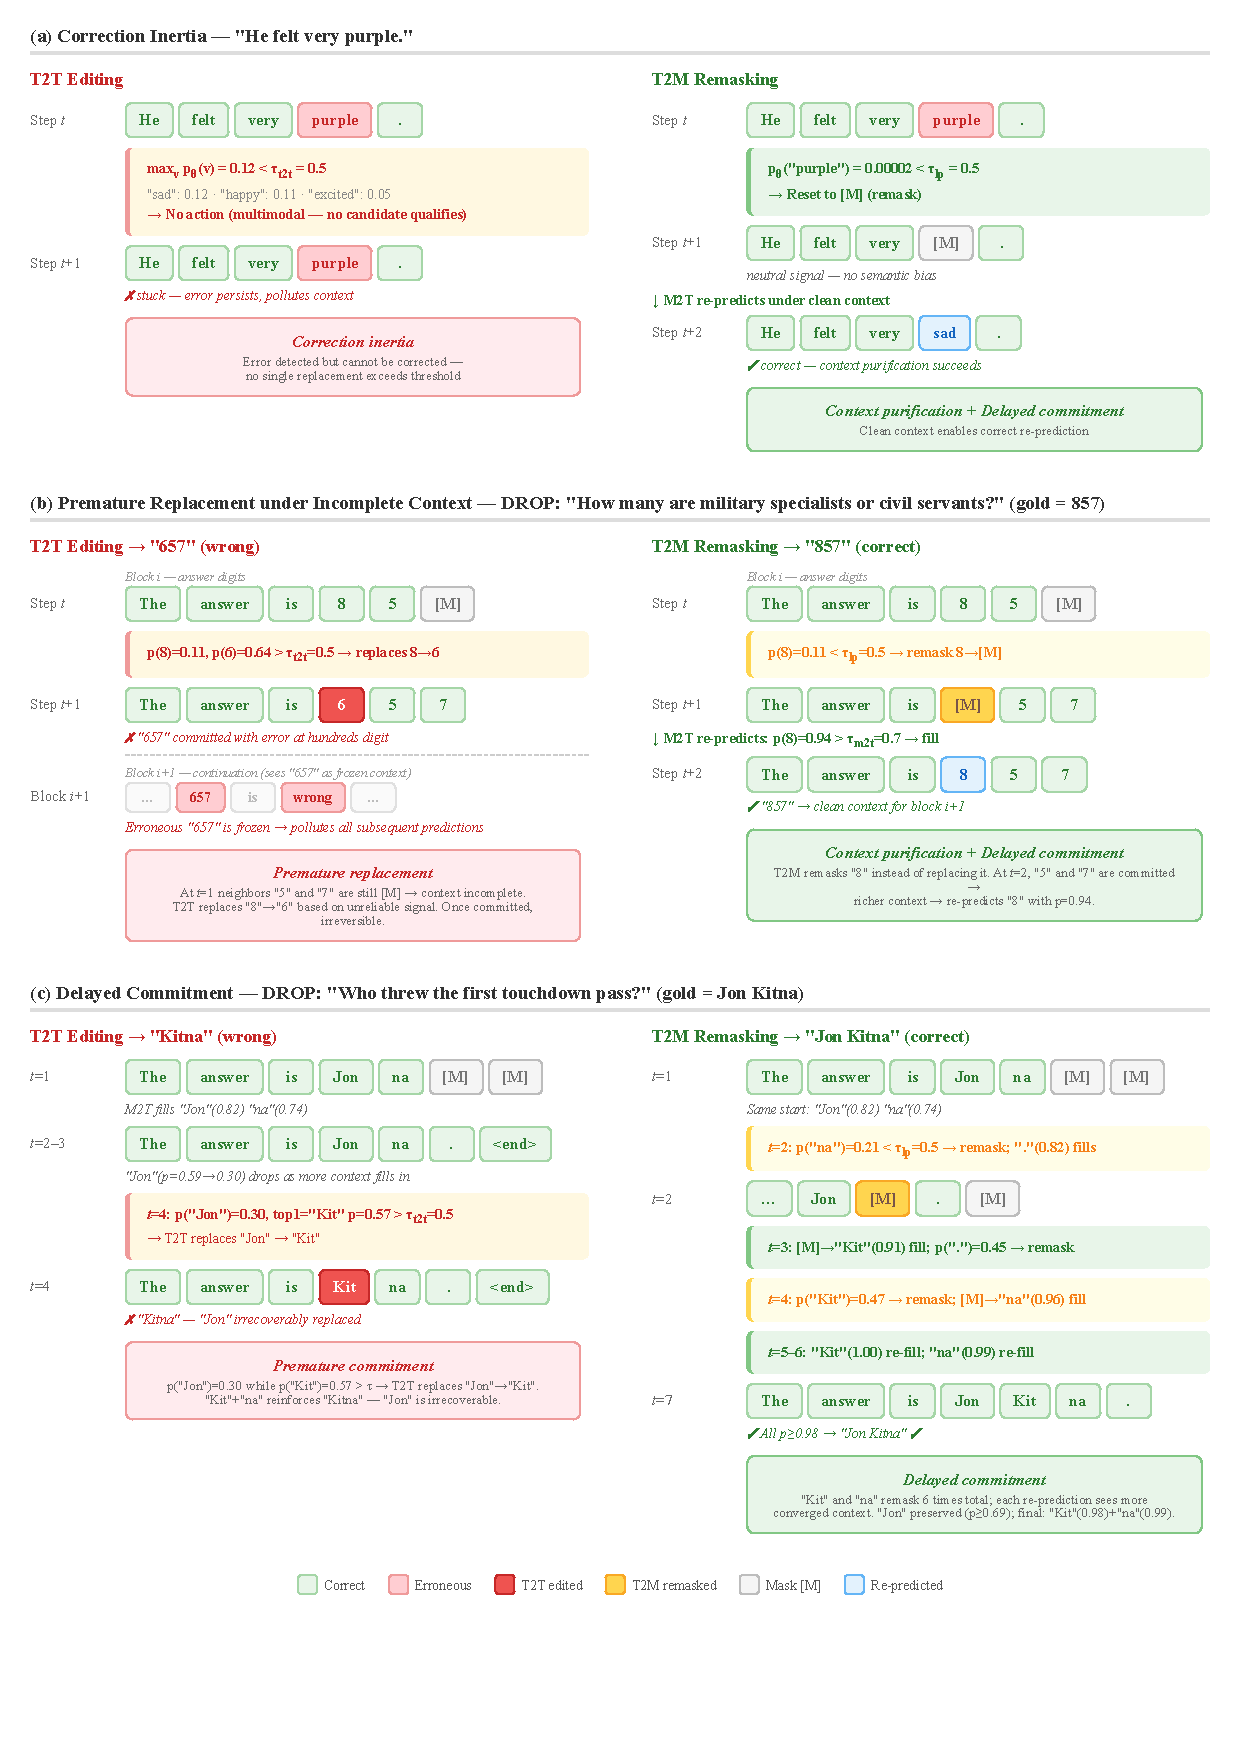
\includegraphics[width=\textwidth, trim=10 60 10 10, clip]{figures/fig1.pdf}
    \caption{\textbf{T2T editing vs.\ T2M remasking.} All probabilities are from LLaDA2.1-mini.
    \textbf{(a)~Correction inertia}: ``He felt very \textcolor{red}{purple}.''---T2T detects the error ($p(\text{purple}){=}0.00002$) but cannot correct it because the distribution is multimodal (``sad'': $0.12$, ``happy'': $0.11$); T2M remasks it and re-predicts correctly.
    \textbf{(b)~Premature replacement} (DROP, gold=857): T2T replaces the initially correct ``8'' ($p{=}0.11$) with ``6'' ($p{=}0.64 {>} \tau_{\text{t2t}}$) under incomplete context; T2M remasks ``8'', waits for context convergence, then re-predicts ``8'' with $p{=}0.94$.
    \textbf{(c)~Delayed commitment} (DROP, gold=Jon Kitna): T2T greedily replaces ``Jon''$\to$``Kit'' ($p{=}0.57$), losing the first name; T2M iteratively remasks uncertain tokens (6 times), preserving ``Jon'' while ``Kit'' and ``na'' converge to $p{\geq}0.98$.}
    \label{fig:overview}
  \end{figure}

\begin{enumerate}
    \item \textbf{Detection--replacement coupling.} \TtoT{} couples error detection and replacement into a single trigger: it fires only when the model assigns probability exceeding $\tau_{\text{t2t}}$ to a token \emph{different} from the current one. In other words, \TtoT{} cannot express ``this token is wrong'' without simultaneously providing ``replace it with this.'' When the conditional distribution is multimodal (multiple plausible tokens sharing probability mass), no single candidate may exceed the threshold, leaving clearly erroneous tokens uncorrected even though the model recognizes them as wrong---a failure mode we term \emph{correction inertia} (Figure~\ref{fig:overview}a).

    \item \textbf{Context pollution} (fundamental limitation of \TtoT{}). \TtoT{}'s core design---replacing one token with another---cannot guarantee context improvement. Even when \TtoT{} is triggered, its replacement is conditioned on context that may itself contain errors at other positions; under such polluted context, even high-confidence replacements may be incorrect. The replaced token, appearing as a legitimate signal, provides misleading semantic cues that bias predictions at all other positions and can create self-reinforcing error cycles (Figures~\ref{fig:overview}b and~\ref{fig:signal}).

    \item \textbf{Train--inference noise mismatch} (limitation of LLaDA2.1's training procedure). LLaDA2.1's \TtoT{} training stream uses \emph{random} token perturbations (uniformly sampled wrong tokens $\to$ ground truth), but at inference time, erroneous tokens are \emph{systematic, model-generated} mistakes that are semantically plausible and correlated with surrounding tokens. This distributional gap means the model encounters a third type of context noise at inference that it has never seen during training---neither the clean \mask{} noise of the \MtoT{} stream nor the random perturbations of the \TtoT{} stream, but systematic, semantically coherent errors from the model itself (see Figure~\ref{fig:signal} for empirical evidence of how such errors mislead predictions).
\end{enumerate}

We propose \emph{Token-to-Mask} (\TtoM{}) remasking as a principled alternative. Instead of replacing suspected tokens, \TtoM{} resets them to the \mask{} state, allowing the diffusion process to re-predict these positions from scratch under a cleaner context. This simple change simultaneously addresses all three limitations: it decouples error detection from replacement, purifies the context by removing erroneous tokens, and converts systematic inference errors back to the model's native \mask{} noise type. Moreover, by reverting to \mask{} rather than immediately committing a replacement, \TtoM{} naturally implements \emph{delayed commitment}---deferring the final token decision to a later step where the surrounding context has further converged, enabling joint re-optimization of multiple suspect positions (Figure~\ref{fig:overview}c). Figure~\ref{fig:overview} illustrates the contrast: \TtoT{} leaves an error in place when no confident replacement exists (\emph{correction inertia}), while \TtoM{} resets it to \mask{} and lets a subsequent \MtoT{} step recover the correct token under purified context.

Our approach is \emph{training-free}---it requires no additional training or architectural modification and works as a drop-in replacement for \TtoT{} within LLaDA2.1's existing generation pipeline. We design and empirically validate three complementary error detection strategies (\textsc{LowProb}, \textsc{T2T-Remask}, and \textsc{LogitDiff}), each targeting a different signal of token unreliability, with thresholds tuned on a small-scale pilot set. We provide a unified theoretical analysis from four perspectives: decoupled detection, context purification, train--inference noise mismatch, and delayed commitment.

Our contributions are:
\begin{itemize}
    \item We identify fundamental limitations of \TtoT{} editing in LLaDA2.1 and propose \TtoM{} remasking as a principled, training-free replacement.
    \item We design and empirically validate three error detection strategies on a small-scale pilot set, and analyze their complementary strengths.
    \item We provide a unified theoretical framework explaining why mask tokens are strictly preferable to erroneous tokens as context, from the perspectives of train--inference noise mismatch, context signal hierarchy, and delayed commitment.
    \item We discover that \emph{last-mile token corruption}---where the model's reasoning is correct but the final answer is corrupted during denoising---is the dominant error mode (79.9\% of errors on CMATH), and show that \TtoM{} specifically repairs this failure mode.
    \item We conduct comprehensive experiments across 12 benchmarks, showing general improvements on tasks requiring precise token-level output, with the largest gain on mathematics.
\end{itemize}


%=============================================================================
\section{Background}
\label{sec:background}
%=============================================================================

\subsection{Masked Diffusion Language Models}

A masked diffusion language model defines a forward noising process that progressively masks tokens and a reverse denoising process that recovers them~\citep{austin2021d3pm,ou2025absorbingdiscrete,sahoo2024mdlm}. Given a clean sequence $\mathbf{x} = (x_1, \ldots, x_L)$, the forward process at time $t \in [0,1]$ independently replaces each token with the mask token \mask{} with probability $\alpha_t$ (where $\alpha_0 = 0$ and $\alpha_1 = 1$), yielding the noisy sequence $\mathbf{z}_t$.

The model $p_\theta(\mathbf{x} \mid \mathbf{z}_t)$ is trained to predict all masked positions simultaneously via a cross-entropy loss:
\begin{equation}
    \mathcal{L}(\theta) = -\mathbb{E}_{\mathbf{x}, t}\left[\frac{1}{\sum_i \mathbbm{1}[z_t^i = \mask{}]} \sum_{i=1}^{L} \mathbbm{1}[z_t^i = \mask{}] \log p_\theta(x_i \mid \mathbf{z}_t)\right].
    \label{eq:mdlm_loss}
\end{equation}

At inference, generation proceeds by starting from a fully masked sequence and iteratively: (1)~predicting all masked positions, (2)~retaining predictions whose confidence exceeds a threshold, subject to a budget cap determined by the unmasking schedule---when more predictions qualify than the budget allows, only the top-$k$ most confident are committed and the rest are remasked~\citep{sahoo2024mdlm}.

\subsection{Block Diffusion}
\label{sec:block_diffusion}

LLaDA2.1~\citep{nie2026llada21} adopts a \emph{semi-autoregressive} block diffusion architecture. The response is divided into blocks of $B$ tokens (typically $B=32$), generated \emph{sequentially} from left to right; within each block, tokens are generated \emph{in parallel} via iterative denoising.

\paragraph{Prompt and response handling.} Given a prompt--response pair, the prompt tokens are placed into the sequence \emph{unmasked}---only the response positions are initialized as \mask{} tokens. In blocks that partially overlap with the prompt, the prompt positions are marked as non-editable and remain frozen throughout generation.

\paragraph{Block-causal attention.} To maintain left-to-right coherence while preserving parallel generation within each block, LLaDA2.1 employs a \emph{block-causal} attention mask. \emph{Within} a block, all positions attend to each other bidirectionally, enabling the model to capture intra-block dependencies. \emph{Across} blocks, attention is strictly causal: block $j$ can attend to blocks $0, 1, \ldots, j$ but not to any future block $j' > j$. This block-level lower-triangular mask is constructed as $\mathbf{M}_{\text{attn}} = \text{tril}(\mathbf{1}_{N_b \times N_b})$ at the block level and expanded to token-level resolution. Previously generated blocks are frozen and their key--value states cached for efficient reuse in subsequent blocks.

\paragraph{Iterative M2T denoising.} Within each block, the model iteratively fills \mask{} positions via Mask-to-Token (\MtoT{}) steps. At each iteration, the model predicts token distributions $p_\theta(x_i \mid \mathbf{z})$ for all masked positions. Positions whose confidence exceeds a threshold $\tau_{\text{m2t}}$ are committed; when fewer positions qualify than the per-step budget $n_{\text{transfer}}$, the top-$n_{\text{transfer}}$ most confident predictions are committed instead. The inner loop repeats until all masks in the block are filled.

\subsection{Token-to-Token (T2T) Editing}
\label{sec:t2t_editing}

Beyond \MtoT{}, LLaDA2.1 introduces a \emph{Token-to-Token} (\TtoT{}) editing phase at each denoising step. For positions already containing committed (non-mask) tokens, the model checks whether a different token is predicted with confidence exceeding $\tau_{\text{t2t}}$. If so, the committed token is \emph{directly replaced}:
\begin{equation}
    x_i \leftarrow x_i^{*} \quad \text{if} \quad p_\theta(x_i^{*} \mid \mathbf{z}) > \tau_{\text{t2t}} \;\land\; x_i^{*} \neq \xold,
    \label{eq:t2t}
\end{equation}
where $x_i^{*} = \arg\max_v p_\theta(v \mid \mathbf{z})$ is the model's top prediction and $\xold$ is the currently committed token. Prompt positions within a block are excluded from \TtoT{} editing.

The inner loop continues until all masks are filled and no further \TtoT{} edits are triggered. Then generation proceeds to the next block, with the current block's tokens frozen as context.

%=============================================================================
\section{Method: Token-to-Mask Remasking}
\label{sec:method}
%=============================================================================

\subsection{Overview}

We replace \TtoT{} editing with \emph{Token-to-Mask} (\TtoM{}) remasking. When the error detection mechanism identifies a committed token as likely incorrect, instead of replacing it with another token, we reset it to \mask{}:
\begin{equation}
    x_i \leftarrow \mask{} \quad \text{if} \quad \textsc{ShouldRemask}(i, \mathbf{z}, \theta),
    \label{eq:t2m}
\end{equation}
and the subsequent \MtoT{} step re-predicts this position with updated context. This is a minimal, surgical change to LLaDA2.1's generation loop: only the token editing phase is replaced (see Algorithm~\ref{alg:t2m}); all other components (model architecture, \MtoT{} logic, block scheduling, KV caching) remain identical.

\subsection{Error Detection Strategies}

We design and empirically validate three complementary strategies for \textsc{ShouldRemask}, each capturing a different signal of token unreliability.

\paragraph{Strategy 1: \textsc{LowProb} --- Current probability is low.}
The model re-evaluates all committed tokens under the current context. If the probability assigned to the currently committed token is low, it is remasked:
\begin{equation}
    \textsc{Remask}_{\textsc{lp}}(i) = \mathbbm{1}\left[p_\theta(\xold \mid \mathbf{z}_{-i}) < \tau_{\text{lp}}\right].
    \label{eq:low_prob}
\end{equation}
This strategy directly tests ``does the model still think this token belongs here?'' without requiring a specific replacement candidate.

\paragraph{Strategy 2: \textsc{T2T-Remask} --- Same trigger, different action.}
This strategy uses the identical triggering condition as \TtoT{} (the model confidently predicts a \emph{different} token), but applies remasking instead of replacement:
\begin{equation}
    \textsc{Remask}_{\textsc{t2t}}(i) = \mathbbm{1}\left[p_\theta(\xnew \mid \mathbf{z}) > \tau_{\text{tr}} \;\land\; \xnew \neq \xold\right].
    \label{eq:t2t_remask}
\end{equation}
By preserving the detection logic but changing the action, this strategy isolates the effect of mask-based correction versus token-based replacement.

\paragraph{Strategy 3: \textsc{LogitDiff} --- Confidence drop.}
This strategy compares the model's outputs from two consecutive denoising iterations within the same block. Let $p_\theta^{(t)}(\cdot \mid \mathbf{z}^{(t)})$ denote the model's prediction at iteration $t$, where the context $\mathbf{z}^{(t)}$ reflects the block state \emph{after} the \MtoT{}/editing updates of iteration $t{-}1$. For a committed token $\xold$ at position $i$, we remask when the model's confidence in that token \emph{drops by more than} $\tau_{\text{ld}}$ between iterations:
\begin{equation}
    \textsc{Remask}_{\textsc{ld}}(i) = \mathbbm{1}\left[p_\theta^{(t-1)}(\xold \mid \mathbf{z}^{(t-1)}) - p_\theta^{(t)}(\xold \mid \mathbf{z}^{(t)}) > \tau_{\text{ld}}\right].
    \label{eq:logit_diff}
\end{equation}
A confidence drop indicates that, as surrounding positions get filled or corrected, the evolving context no longer supports this token---a signal that it is inconsistent with its converging neighborhood. An increase in confidence, conversely, means the token is being validated by the evolving context and should be kept. Unlike \textsc{LowProb} which uses a single-step snapshot, \textsc{LogitDiff} captures \emph{dynamic} context evolution across iterations. On the first iteration of each block, no previous logits exist, so no remasking is triggered.

\subsection{Safety Mechanisms}

Unrestricted remasking could lead to oscillation (repeatedly remasking and re-predicting the same positions). We employ two safeguards:

\paragraph{Per-position remask budget.} Each position $i$ maintains a counter $c_i$, incremented each time it is remasked. Remasking is blocked when $c_i \geq C_{\max}$ (default $C_{\max} = 1$), preventing infinite cycles.

\paragraph{Remask ratio cap.} At each step, at most a fraction $\rho_{\max}$ (default $\rho_{\max} = 0.25$) of editable positions may be remasked. When more positions are flagged, we prioritize those with the lowest confidence scores (strategy-dependent), ensuring the most suspect tokens are addressed first.

\begin{algorithm}[t]
\caption{Token-to-Mask (\TtoM{}) Remasking (replacing \TtoT{} editing in LLaDA2.1)}
\label{alg:t2m}
\begin{algorithmic}[1]
\REQUIRE Current block tokens $\mathbf{z}$, model $p_\theta$, mask id \mask{}, strategy $\mathcal{S}$, threshold $\tau$, budget $C_{\max}$, ratio cap $\rho_{\max}$
\STATE \textbf{// Standard M2T step (unchanged from LLaDA2.1)}
\FOR{each mask position $i$ where $z_i = \mask{}$}
    \IF{$\max_v p_\theta(v \mid \mathbf{z}) > \tau_{\text{m2t}}$}
        \STATE $z_i \leftarrow \arg\max_v p_\theta(v \mid \mathbf{z})$
    \ENDIF
\ENDFOR
\STATE
\STATE \textbf{// T2M remasking step (replaces T2T editing)}
\STATE $\mathcal{E} \leftarrow \{i : z_i \neq \mask{} \text{ and } i \notin \text{prompt}\}$ \hfill $\triangleright$ editable positions
\STATE $\mathcal{R} \leftarrow \{i \in \mathcal{E} : \textsc{ShouldRemask}_\mathcal{S}(i, \mathbf{z}, \tau) \text{ and } c_i < C_{\max}\}$
\IF{$|\mathcal{R}| > \rho_{\max} \cdot |\mathcal{E}|$}
    \STATE $\mathcal{R} \leftarrow \text{top-}k \text{ by lowest confidence score, } k = \lfloor \rho_{\max} \cdot |\mathcal{E}| \rfloor$
\ENDIF
\FOR{each $i \in \mathcal{R}$}
    \STATE $z_i \leftarrow \mask{}$; \quad $c_i \leftarrow c_i + 1$
\ENDFOR
\STATE \textbf{return} $\mathcal{R} = \emptyset$ \hfill $\triangleright$ converged if no remasking occurred
\end{algorithmic}
\end{algorithm}

%=============================================================================
\section{Theoretical Analysis}
\label{sec:theory}
%=============================================================================

We provide a unified theoretical framework for understanding why \TtoM{} remasking is preferable to \TtoT{} editing. Our analysis proceeds along four complementary axes.

\subsection{Decoupling Error Detection from Correction}

\TtoT{} editing couples two logically independent decisions into a single condition: (1)~\emph{Is the current token wrong?} and (2)~\emph{Is there a confident replacement?} This coupling creates \emph{correction inertia}: despite clear evidence that a token is erroneous, the system cannot initiate correction because no single replacement meets the confidence threshold. We formalize this via the \emph{stuck set}:

\begin{definition}[Stuck set]
The stuck set $\Sstuck$ contains positions where the current token is likely wrong but no single replacement exceeds the confidence threshold:
\begin{equation}
    \Sstuck = \left\{i : p_\theta(\xold \mid \mathbf{z}_{-i}) < \epsilon, \;\text{but}\; \max_v p_\theta(v \mid \mathbf{z}_{-i}) < \tau_{\text{t2t}}\right\}.
    \label{eq:stuck}
\end{equation}
\end{definition}

\noindent This situation arises naturally when the conditional distribution $p_\theta(\cdot \mid \mathbf{z}_{-i})$ is multimodal. For instance, consider completing ``He felt very \underline{\hspace{1cm}}.''\ with LLaDA2.1-mini: the tokens ``sad,'' ``happy,'' and ``excited'' receive probabilities $0.12$, $0.11$, and $0.05$ respectively (Figure~\ref{fig:overview}), while the incorrect committed token ``purple'' has probability ${\sim}0.00002$. \TtoT{} with $\tau_{\text{t2t}} = 0.5$ takes no action since $\max_v p_\theta(v) = 0.12 < 0.5$, despite the model clearly recognizing the error.

\noindent \TtoT{} is completely ineffective on $\Sstuck$: its trigger requires $\max_v p_\theta(v \mid \mathbf{z}_{-i}) > \tau_{\text{t2t}}$, which fails by definition of $\Sstuck$. In contrast, \textsc{LowProb} only checks whether $p_\theta(\xold \mid \mathbf{z}_{-i}) < \tau_{\textsc{lp}}$---it does not require high confidence in any specific replacement. Since $p_\theta(\xold \mid \mathbf{z}_{-i}) < \epsilon \ll \tau_{\textsc{lp}}$ for positions in $\Sstuck$, \textsc{LowProb} necessarily triggers remasking, handing these positions to the subsequent \MtoT{} step for re-prediction under potentially more converged context. Note that remasking is a \emph{necessary} step for initiating correction but does not guarantee a correct re-prediction---the key point is that \TtoT{} cannot even take this first step.

\subsection{Error Context Purification}

The most critical advantage of \TtoM{} concerns the quality of the \emph{context} under which re-prediction occurs. In iterative denoising, the model's prediction at position $i$ is conditioned on all other positions:
\begin{equation}
    p_\theta(x_i \mid \mathbf{z}_{-i}) = p_\theta\!\left(x_i \mid \underbrace{\mathbf{z}_{\text{correct}}}_{\text{correct tokens}},\; \underbrace{\mathbf{z}_{\text{error}}}_{\text{wrong tokens}},\; \underbrace{\mask{}, \ldots, \mask{}}_{\text{unknown}}\right).
\end{equation}

\paragraph{Erroneous tokens in context.} In parallel generation, errors are inevitable: \MtoT{} may fill a mask position with an incorrect token, and \TtoT{} may replace a token with another that is also wrong. These erroneous tokens---regardless of their source---appear as legitimate tokens in the context, providing misleading semantic signals that bias predictions at all other positions. The key question is: when an error is detected, what should be done with the position?

\paragraph{T2T: Replace with another token.} \TtoT{} substitutes the suspected error with the model's current top prediction. However, even when this replacement has high confidence, the model's prediction is conditioned on context that may itself contain errors at other positions---under a polluted context, high confidence does not imply high correctness. Consequently, the replacement may itself be incorrect, and the erroneous token remains in the context as a seemingly legitimate signal, biasing not only subsequent predictions at \emph{other} positions but also the re-evaluation of this \emph{same} position in later iterations, creating a self-reinforcing error cycle.

\paragraph{T2M: Reset to neutral mask.} \TtoM{} replaces suspected errors with \mask{}, which the model recognizes as ``unknown.'' Mask tokens carry no semantic bias---they are entirely neutral, neither misleading predictions at other positions nor interfering with re-prediction at the reset position itself. By progressively replacing detected errors with \mask{}, the proportion of correct tokens and neutral masks in the context increases while misleading signals are correspondingly reduced.

\begin{remark}[Context signal hierarchy]
\label{rem:signal}
For predicting position $i$, each context position $j \neq i$ provides one of three types of signals:
\begin{enumerate}
    \item \textbf{Aligned signal} ($z_j = x_j^{*}$, correct token): biases $p_\theta(x_i \mid \mathbf{z})$ toward the correct $x_i^{*}$, as the model leverages correct semantic dependencies.
    \item \textbf{Null signal} ($z_j = \mask{}$): does not bias $p_\theta(x_i \mid \mathbf{z})$ in any semantic direction. The model, having been trained extensively on masked contexts, produces calibrated predictions that effectively marginalize over the unknown position.
    \item \textbf{Adversarial signal} ($z_j = e_j \neq x_j^{*}$, erroneous token): biases $p_\theta(x_i \mid \mathbf{z})$ \emph{away} from $x_i^{*}$. The model cannot distinguish $e_j$ from a correct token, so it trusts the wrong semantic signal and adjusts its prediction accordingly.
\end{enumerate}
\end{remark}

Under this hierarchy, \TtoM{} replaces type~(3) signals with type~(2), eliminating sources of adversarial bias at zero cost (null signals are strictly non-harmful). \TtoT{} replaces type~(3) with a new token that may itself be type~(3), providing no guarantee of net improvement. Figure~\ref{fig:signal} provides empirical verification: we construct ``I went to \underline{\hspace{1cm}} and visited the \mask{} Tower.'' with four context variants and measure the model's prediction at the \mask{} position. With the correct token ``France,'' the model predicts ``Eiffel'' ($p{=}0.97$). With \mask{}, the prediction is preserved (``Eiffel,'' $p{=}0.82$) but less confident. With the semantically related error ``Japan,'' the model is \emph{actively misled} to predict ``Tokyo'' ($p{=}0.91$)---a high-confidence wrong answer. This demonstrates that adversarial signals are strictly worse than null signals, and that \TtoM{}'s conversion of adversarial$\to$null is always safe.

\begin{figure}[htp]
    \centering
    % trim={left bottom right top}, 单位pt，可自行调整
    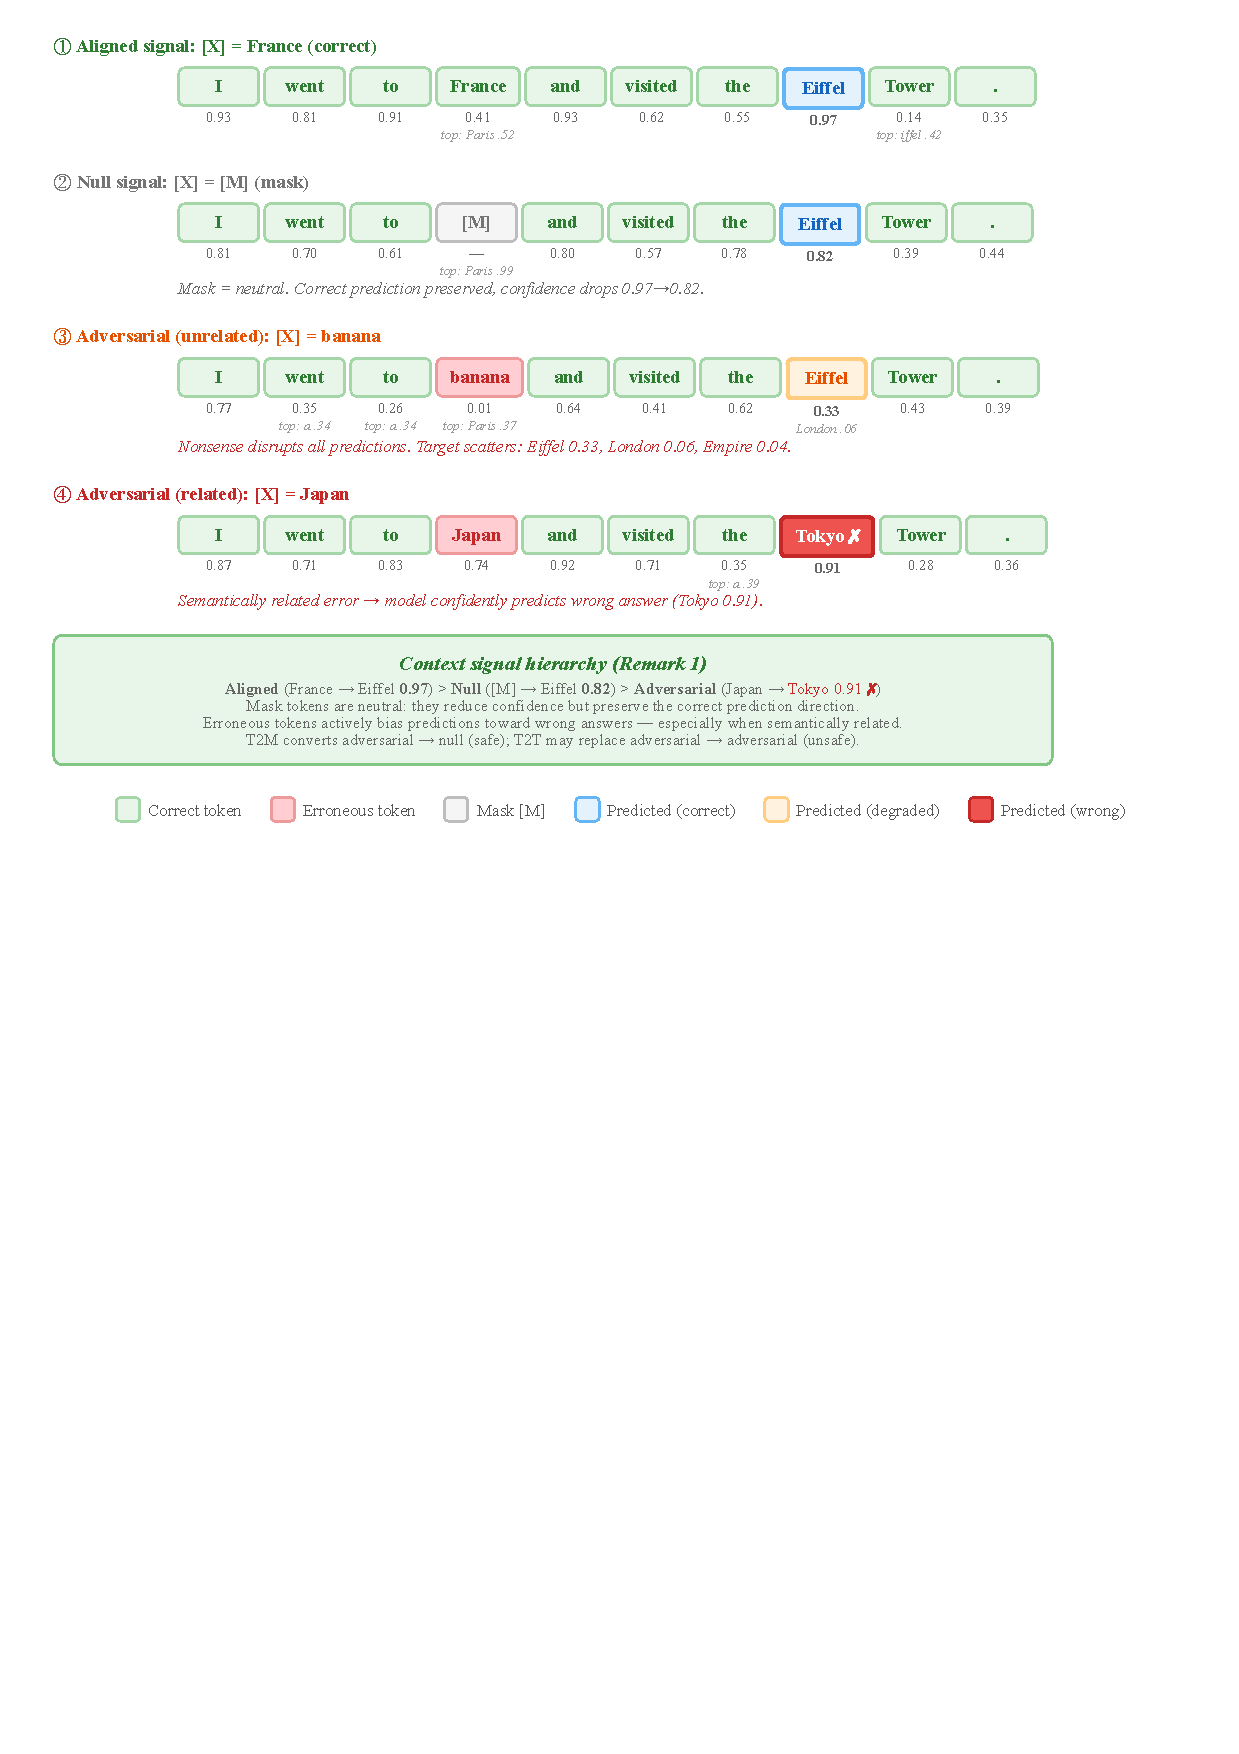
\includegraphics[width=\textwidth, trim=20 440 20 10, clip]{figures/fig2_signal.pdf}
    \caption{\textbf{Empirical verification of context signal hierarchy} (Remark~\ref{rem:signal}) on LLaDA2.1-mini. We vary a single context position [X] in ``I went to [X] and visited the \mask{} Tower'' and measure predictions at the \mask{} position. Aligned context (France) yields a confident correct prediction ($p(\text{Eiffel}){=}0.97$). Null context (\mask{}) preserves correctness at reduced confidence ($0.82$). Adversarial context (Japan) \emph{actively misleads} the model to a wrong answer ($p(\text{Tokyo}){=}0.91$). Unrelated noise (banana) degrades confidence without directing to a specific wrong answer ($p(\text{Eiffel}){=}0.33$). This confirms: aligned $>$ null $>$ adversarial, justifying \TtoM{}'s adversarial$\to$null conversion.}
    \label{fig:signal}
\end{figure}

\paragraph{Error propagation cycle.} When multiple adversarial signals coexist, they interact: an error at position $j$ biases the prediction at position $i$, which in turn reinforces the error at $j$ in subsequent iterations. This mutual reinforcement can converge to a \emph{stable but incorrect fixed point}. \TtoM{} breaks this cycle by simultaneously converting multiple adversarial signals to null signals, severing the inter-position error dependencies.

\subsection{Train--Inference Noise Mismatch}

LLaDA2.1 employs a dual-stream training objective~\citep{nie2026llada21}: the \MtoT{} stream trains the model to predict correct tokens from masked context; the \TtoT{} stream trains the model to recover ground-truth tokens from randomly perturbed positions (random wrong token $\to$ ground truth). The model has thus encountered both \mask{} noise and random-token noise during training. However, there is a critical distributional gap between training noise and inference errors.

\paragraph{Random perturbations $\neq$ systematic errors.} During \TtoT{} training, the perturbed tokens are sampled \emph{uniformly at random} from the vocabulary---they are uncorrelated with the context and semantically incoherent. At inference time, however, erroneous tokens are \emph{systematic, model-generated} mistakes that are often semantically plausible, locally coherent, and correlated with surrounding tokens. This gap affects \emph{both} \MtoT{} and \TtoT{} operations: regardless of the operation type, the non-mask context during inference may contain model-generated errors whose distribution differs fundamentally from anything seen during training.

\paragraph{Mask as a strictly safer context signal.} Given this mismatch, what is the best action when an error is detected? Mask tokens carry strictly less misleading information than erroneous tokens: a mask communicates ``unknown,'' whereas an erroneous token actively provides a false semantic signal. By converting suspected errors to \mask{}:
\begin{equation}
    \underbrace{\{\mathbf{z}_{\text{correct}}, \mathbf{z}_{\text{error}}\}}_{\text{context with errors}} \xrightarrow{\text{T2M}} \underbrace{\{\mathbf{z}_{\text{correct}}, \mask{}\}}_{\text{cleaner context}},
\end{equation}
\TtoM{} replaces actively misleading signals with neutral ``unknown'' markers, converting the context back to a form the model handles most reliably. Figure~\ref{fig:signal} illustrates this mismatch concretely: random perturbations during \TtoT{} training resemble ``banana'' replacing ``France''---semantically incoherent noise that merely degrades confidence ($p(\text{Eiffel}){=}0.33$) without directional bias. In contrast, actual inference-time errors resemble ``Japan'' replacing ``France''---semantically related, locally coherent errors that \emph{actively mislead} the model toward high-confidence wrong predictions ($p(\text{Tokyo}){=}0.91$). This distributional gap is the essence of the train--inference mismatch. \mask{} avoids both failure modes entirely ($p(\text{Eiffel}){=}0.82$).

\paragraph{Analogy with continuous diffusion.} In continuous diffusion models~\citep{ho2020ddpm,song2021scorebased}, the denoising score function $\nabla_{\mathbf{x}} \log p(\mathbf{x})$ is trained with Gaussian noise. If the noise distribution at test time deviates from the training distribution (e.g., structured adversarial perturbations instead of random Gaussian noise), score estimation degrades. Analogously, in masked diffusion, the model is trained with two noise types: \mask{} tokens (\MtoT{}) and random token perturbations (\TtoT{}). Inference-time errors---systematic, correlated, semantically plausible---constitute a third, unseen noise type (see Figure~\ref{fig:signal}). \TtoM{} addresses this by converting the unseen noise back to the familiar \mask{} type.

\subsection{Delayed Commitment and Joint Optimization}

\TtoT{} is a \emph{greedy} strategy: once it identifies a high-confidence alternative, it immediately commits. This greedy commitment has two problems:

\begin{enumerate}
    \item \textbf{Premature locking.} The replacement token, once committed, becomes context for all other positions. If the replacement is itself suboptimal (e.g., the argmax under multimodal distributions), this error propagates irreversibly.
    \item \textbf{Per-position independence.} \TtoT{} optimizes each position independently: $\hat{x}_i = \arg\max p_\theta(x_i \mid \mathbf{z}_{-i})$. This ignores inter-position dependencies.
\end{enumerate}

\TtoM{} implements \emph{delayed commitment}: by resetting suspect positions to \mask{}, it defers the final decision to a later step where more context has converged. When multiple positions are simultaneously remasked, the subsequent \MtoT{} step effectively solves a \emph{joint} optimization:
\begin{equation}
    \hat{\mathbf{x}}_{\mathcal{R}} = \arg\max_{\mathbf{x}_{\mathcal{R}}} \prod_{i \in \mathcal{R}} p_\theta(x_i \mid \mathbf{z}_{\text{correct}}, \mask{}^{|\mathcal{R}|}),
\end{equation}
where $\mathcal{R}$ is the set of remasked positions. While the prediction at each position is still independent conditional on the context, the context itself is \emph{jointly cleaner} (all errors in $\mathcal{R}$ are simultaneously removed), yielding better individual predictions that are more globally consistent.

This is analogous to \emph{simulated annealing}: \TtoM{} locally increases uncertainty (remasking) to escape local optima and explore more globally optimal solutions.

\paragraph{Illustrative examples.} Figure~\ref{fig:overview}(b) demonstrates premature locking on a DROP example (gold answer = 857). At an early denoising step, when only ``8'' ($p{=}0.11$) has been committed while ``5'' and ``7'' are still \mask{}, \TtoT{} greedily replaces ``8'' with ``6'' ($p{=}0.64 > \tau_{\text{t2t}}$) based on incomplete context, producing the wrong answer 657. \TtoM{} instead remasks ``8'', waits for ``5'' and ``7'' to be committed, and then re-predicts ``8'' with $p{=}0.94$ under fully converged context.

Figure~\ref{fig:overview}(c) illustrates joint multi-position optimization on a DROP example (gold = ``Jon Kitna''). \TtoT{} greedily replaces ``Jon''$\to$``Kit'' ($p{=}0.57$), destroying the first name. \TtoM{} iteratively remasks uncertain tokens (6 rounds), allowing ``Jon'' to remain stable while ``Kit'' and ``na'' gradually converge to $p{\geq}0.98$---the system finds a globally consistent solution by deferring commitment across multiple interdependent positions.

%=============================================================================
\section{Related Work}
\label{sec:related}
%=============================================================================

\paragraph{Discrete masked diffusion language models.}
Masked diffusion models for text generation have advanced rapidly. D3PM~\citep{austin2021d3pm} introduced discrete diffusion with absorbing states. MDLM~\citep{sahoo2024mdlm} and SEDD~\citep{lou2024sedd} developed efficient training objectives. LLaDA~\citep{nie2025llada} scaled to 8B parameters with competitive performance, and LLaDA2.1~\citep{nie2026llada21} introduced \TtoT{} editing for faster inference. Dream~\citep{ye2025dream} further demonstrated the viability of diffusion LMs at scale.

\paragraph{Remasking in masked diffusion.}
ReMDM~\citep{wang2025remdm} is the pioneering work on remasking for masked diffusion. It modifies the reverse posterior to introduce a \emph{probabilistic} remasking parameter $\sigma_t$, allowing any unmasked token to be randomly remasked at each step. ReMDM operates at the \emph{sampling process level}, modifying the entire reverse diffusion trajectory. In contrast, our approach operates specifically at the \emph{editing step level} within LLaDA2.1, performing \emph{targeted} remasking based on explicit error detection rather than random remasking.

Using the signal hierarchy of Remark~\ref{rem:signal}, we can formalize why targeted remasking is strictly preferable. Consider $N$ committed (non-mask) positions, of which $N_c$ are correct (aligned signal, value $s_+ > 0$) and $N_e$ are erroneous (adversarial signal, cost $s_- < 0$). Define context quality as $Q = N_c \cdot s_+ + N_e \cdot s_-$. Under \textbf{random remasking} with per-token probability $\sigma$, each position is independently remasked regardless of correctness:
\begin{equation}
    Q_{\text{random}}(\sigma) = (1 - \sigma)(N_c \cdot s_+ + N_e \cdot s_-).
    \label{eq:q_random}
\end{equation}
This creates an inherent dilemma: increasing $\sigma$ removes adversarial signals but \emph{equally} destroys aligned signals. Under \textbf{targeted remasking} (assuming perfect detection), only the $N_e$ erroneous positions are remasked:
\begin{equation}
    Q_{\text{targeted}} = N_c \cdot s_+.
    \label{eq:q_targeted}
\end{equation}
The advantage of targeted over random remasking is:
\begin{equation}
    Q_{\text{targeted}} - Q_{\text{random}}(\sigma) = \underbrace{\sigma \cdot N_c \cdot s_+}_{\text{aligned signals preserved}} + \underbrace{(1 - \sigma)(-N_e \cdot s_-)}_{\text{adversarial signals removed}} > 0
    \label{eq:q_advantage}
\end{equation}
for all $\sigma \in (0, 1]$. Both terms are strictly positive: targeted remasking simultaneously preserves more correct context and removes more errors. Even with imperfect detection, targeted remasking outperforms random remasking as long as the detector is better than chance, i.e., its precision-recall tradeoff exceeds the base rate $N_e / N$.

CORE~\citep{zhai2026core} proposes context-robust remasking that identifies ``context-brittle'' tokens via sensitivity to masked perturbations, arguing that static probability-based heuristics are myopic. However, we note a potential limitation of the sensitivity-based approach. CORE's sensitivity metric measures conditional mutual information $I(X_i; Z_S \mid Z_{-i,-S})$, which may be influenced by the \emph{current mask pattern} of the denoising state rather than token correctness alone. For instance, a correct token may exhibit low sensitivity when its semantically related neighbors are still \mask{} (the relevant context is already absent), yet the same token's sensitivity may spike once those neighbors are filled---regardless of whether the fill is correct. Conversely, an erroneous token may appear ``stable'' simply because its correlated neighbors happen to be unpredicted. This suggests that CORE's sensitivity may partly reflect the \emph{transient state of the denoising process} (which positions happen to be filled) rather than the intrinsic correctness of the token.

In contrast, the static probability $p_\theta(x_i \mid \mathbf{z})$ is the model's \emph{posterior belief} about $x_i$ given the \emph{full} current context---arguably the most direct available signal for token correctness. By the data processing inequality, evaluating under artificially degraded context (CORE's masking perturbations) cannot yield strictly more information about $X_i$'s correctness than the full-context prediction.

Practically, CORE requires $O(k)$ additional forward passes per perturbation test, while static probability is a free byproduct of the existing forward pass. Our \textsc{LogitDiff} strategy captures a related but more principled form of sensitivity: it tracks how the model's opinion changes along the \emph{actual} denoising trajectory rather than under artificial perturbations, also at zero extra forward-pass cost.

\paragraph{Training-based correction.}
Several methods improve remasking quality through additional training. RemeDi~\citep{remedi2025} trains a dual-stream architecture with supervised fine-tuning and reinforcement learning to learn per-token confidence scores for remasking decisions. ProSeCo~\citep{schiff2026proseco} adds a corrector cross-entropy loss to train the model to recover from its own mistakes. PRISM~\citep{kim2025prism} attaches a lightweight adapter fine-tuned with a self-correction loss. MDPO~\citep{he2025mdpo} frames denoising as sequential decision-making and applies policy optimization, also proposing Running Confidence Remasking (RCR) as a training-free baseline. These methods are complementary to our approach: they improve the model's ability to detect or correct errors through training, while we improve the \emph{correction mechanism} itself (T2M vs.\ T2T) without any training.

\paragraph{Positioning.}
Our approach offers principled advantages over existing remasking methods along three axes. \emph{Compared with ReMDM}, we replace blind random remasking with targeted error-driven remasking, which we formally show to be strictly superior in context quality (Eq.~\ref{eq:q_random}--\ref{eq:q_advantage}). \emph{Compared with CORE}, we use direct posterior probability and natural denoising-trajectory dynamics (\textsc{LogitDiff}), both grounded in the model's full-context prediction, rather than perturbation-based sensitivity metrics that may be influenced by the transient mask pattern. \emph{Compared with training-based methods} (RemeDi, ProSeCo, PRISM, MDPO), we achieve improvements at zero training cost by addressing the correction mechanism itself (T2M vs.\ T2T) rather than learning better error detectors. Our theoretical framework---the signal hierarchy (Remark~\ref{rem:signal}), the targeted-vs-random analysis, and the delayed commitment formulation---provides a unified foundation that is complementary to and composable with all of the above.

%=============================================================================
\section{Experiments}
\label{sec:experiments}
%=============================================================================

\subsection{Experimental Setup}

\paragraph{Model.} We use LLaDA2.1-mini (16B parameters)~\citep{nie2026llada21}, a Mixture-of-Experts masked diffusion language model. All experiments use the same pretrained checkpoint with no additional training.

\paragraph{Inference hyperparameters.} We adopt LLaDA2.1's recommended Quality Mode (Q Mode) settings: M2T confidence threshold $\tau_{\text{m2t}} = 0.7$, T2T editing threshold $\tau_{\text{t2t}} = 0.5$, block length $B = 32$, temperature $= 0.0$ (greedy), and $\texttt{eos\_early\_stop} = \text{True}$. Generation length is set per-benchmark (see Appendix~\ref{app:benchmarks}).

\paragraph{Remask hyperparameters.} For the main results, we use \TtoM{} with the \textsc{LowProb} strategy ($\tau_{\textsc{lp}} = 0.3$, $C_{\max} = 1$, $\rho_{\max} = 0.25$), selected as the most cost-efficient configuration from the ablation study (Figure~\ref{fig:ablation}). The full hyperparameter sweep across all three strategies is presented in the ablation.

\paragraph{Baselines.} Our primary comparison is between the original \TtoT{} editing (``Original'') and \TtoM{} remasking with the configuration described above. All methods use the same model and inference parameters, isolating the effect of the editing mechanism.

\paragraph{Evaluation note.} We use the official LLaDA2.1 model weights, the HuggingFace-provided inference code, and official benchmark datasets. As LLaDA2.1 does not release its evaluation code, our reproduced baseline absolute scores may differ from the original paper due to prompt template or answer extraction differences; all \TtoT{} vs.\ \TtoM{} comparisons use \emph{identical} evaluation pipelines.

\paragraph{Benchmarks.} We evaluate on 12 benchmarks spanning five categories: \textbf{Knowledge} (GPQA-Diamond~\citep{rein2024gpqa}, TriviaQA~\citep{joshi2017triviaqa}, MMLU-Pro~\citep{wang2024mmlu_pro}), \textbf{Reasoning} (HellaSwag~\citep{zellers2019hellaswag}, PIQA~\citep{bisk2020piqa}, DROP~\citep{dua2019drop}, BBH~\citep{suzgun2023bbh}), \textbf{Mathematics} (CMATH~\citep{wei2023cmath}, AIME~2025~\citep{aime2025}, GSM~Plus~\citep{li2024gsm_plus}), \textbf{Coding} (HumanEval+~\citep{chen2021humaneval,liu2023evalplus}), and \textbf{Instruction Following} (IFEval~\citep{zhou2023ifeval}).

\subsection{Main Results}

\begin{table}[t]
\centering
\caption{Main results across 12 benchmarks. All methods use LLaDA2.1-mini with identical inference parameters. T2M uses \textsc{LowProb} ($\tau{=}0.3$, $C_{\max}{=}1$, $\rho_{\max}{=}0.25$). TriviaQA and DROP report F1; others report accuracy or pass@1 (\%). Best per-benchmark in \textbf{bold}.}
\label{tab:main}
\vspace{4pt}
\small
\begin{tabular}{llcc}
\toprule
\textbf{Category} & \textbf{Benchmark} & \textbf{Original (T2T)} & \textbf{T2M} \\
\midrule
\multirow{3}{*}{Knowledge}
  & GPQA-Diamond   & \textbf{21.72} & \textbf{21.72} \\
  & TriviaQA (F1)  & 30.54          & \textbf{30.96} \\
  & MMLU-Pro       & 58.78          & \textbf{58.84} \\
\midrule
\multirow{4}{*}{Reasoning}
  & HellaSwag      & 78.57          & \textbf{78.67} \\
  & PIQA           & \textbf{82.37} & 81.94          \\
  & DROP (F1)      & 38.53          & \textbf{38.90} \\
  & BBH            & \textbf{75.50} & 75.38          \\
\midrule
\multirow{3}{*}{Math}
  & CMATH          & 82.33          & \textbf{88.25} \\
  & AIME 2025      & \textbf{33.33} & \textbf{33.33} \\
  & GSM Plus       & \textbf{67.54} & 67.21          \\
\midrule
Coding
  & HumanEval+     & \textbf{64.00} & 61.00          \\
\midrule
Instruction
  & IFEval (Strict) & 73.01         & \textbf{74.12} \\
\bottomrule
\end{tabular}
\end{table}

Table~\ref{tab:main} presents the main results. \TtoM{} remasking yields the largest gain on \textbf{CMATH} ($+5.92$), a Chinese elementary math benchmark where final answers are exact numbers and even a single corrupted digit causes failure. Notable improvement is also observed on \textbf{instruction following} (IFEval $+1.1$), where precise format compliance benefits from cleaner context. Modest gains appear on \textbf{extractive QA} (TriviaQA $+0.42$ F1, DROP $+0.37$ F1), where answers are short spans requiring precise token-level reproduction. On \textbf{knowledge} (GPQA $\pm 0.00$, MMLU-Pro $+0.06$), other \textbf{mathematics} benchmarks (AIME~2025 $\pm 0.00$ with only 30 problems, GSM~Plus $-0.33$), and \textbf{commonsense/structured reasoning} (HellaSwag $+0.10$, PIQA $-0.43$, BBH $-0.12$), performance is essentially unchanged. On \textbf{coding} (HumanEval+ $-3.0$), performance decreases, likely because remasking disrupts the syntactic token dependencies that code generation relies on---correct code tokens may appear low-confidence in isolation yet be essential for structural validity. We analyze these task-dependent patterns in Section~\ref{sec:analysis}.

\subsection{Ablation Studies}

\paragraph{Hyperparameter ablation: cost--accuracy trade-off.}
We conduct a full cross-ablation of all hyperparameters on CMATH. We randomly sample 100 problems from the CMATH test set (1,098 problems, fixed seed=42) and run single-sample greedy inference (batch size 1, temperature 0) on a single A100-80GB GPU per configuration. All shared inference parameters follow the Q~Mode defaults from our main experiments: M2T confidence threshold $\tau_{\text{m2t}}{=}0.7$, T2T editing threshold $\tau_{\text{t2t}}{=}0.5$, block length $B{=}32$, generation length 16,384.

The M2T fill threshold $\tau_{\text{m2t}}{=}0.7$ is shared by all configurations (including the baseline), controlling when mask positions are filled. On top of this, we sweep three remask-specific hyperparameters:
\begin{enumerate}[nosep,leftmargin=*]
    \item The \emph{remask threshold} $\tau$ controls how aggressively each strategy triggers remasking. The direction of $\tau$ varies by strategy (Table~\ref{tab:tau_dir}).
    \begin{table}[h]
    \centering\small
    \vspace{-2pt}
    \begin{tabular}{lcl}
    \toprule
    \textbf{Strategy} & \textbf{Higher $\tau$ $\to$} & \textbf{Sweep range} \\
    \midrule
    \textsc{LowProb}    & more remasking & $\{0.1, 0.3, 0.5, 0.7, 0.9\}$ \\
    \textsc{T2T-Remask} & less remasking & $\{0.5, 0.7, 0.9\}$ \\
    \textsc{LogitDiff}  & less remasking & $\{0.1, 0.2, 0.3, 0.5\}$ \\
    \bottomrule
    \end{tabular}
    \caption{Effect of increasing $\tau$ on remask volume per strategy.}
    \label{tab:tau_dir}
    \vspace{-6pt}
    \end{table}
    \item The \emph{per-position budget} $C_{\max} \in \{1, 3, 5\}$ limits how many times each position can be remasked---larger values allow more repeated corrections.
    \item The \emph{ratio cap} $\rho_{\max} \in \{0.25, 0.50, 1.0\}$ limits the fraction of editable positions remasked per step---$1.0$ means no cap.
\end{enumerate}
The baseline uses the original T2T editing with $\tau_{\text{t2t}}{=}0.5$ (no remasking), with all inference parameters aligned with the official LLaDA2.1-mini Q~Mode defaults~\citep{nie2026llada21}. This yields $1 + (5{+}3{+}4) \times 3 \times 3 = 109$ configurations, all evaluated on the same 100 samples.

Figure~\ref{fig:ablation} plots each configuration as a point. The $x$-axis measures average token modifications per sample---T2T edits for the baseline (${\star}$, $\tau_{\text{t2t}}{=}0.5$, 12.4 edits/sample), remask count for \TtoM{} strategies. The $y$-axis measures accuracy.

\begin{figure}[htp]
    \centering
    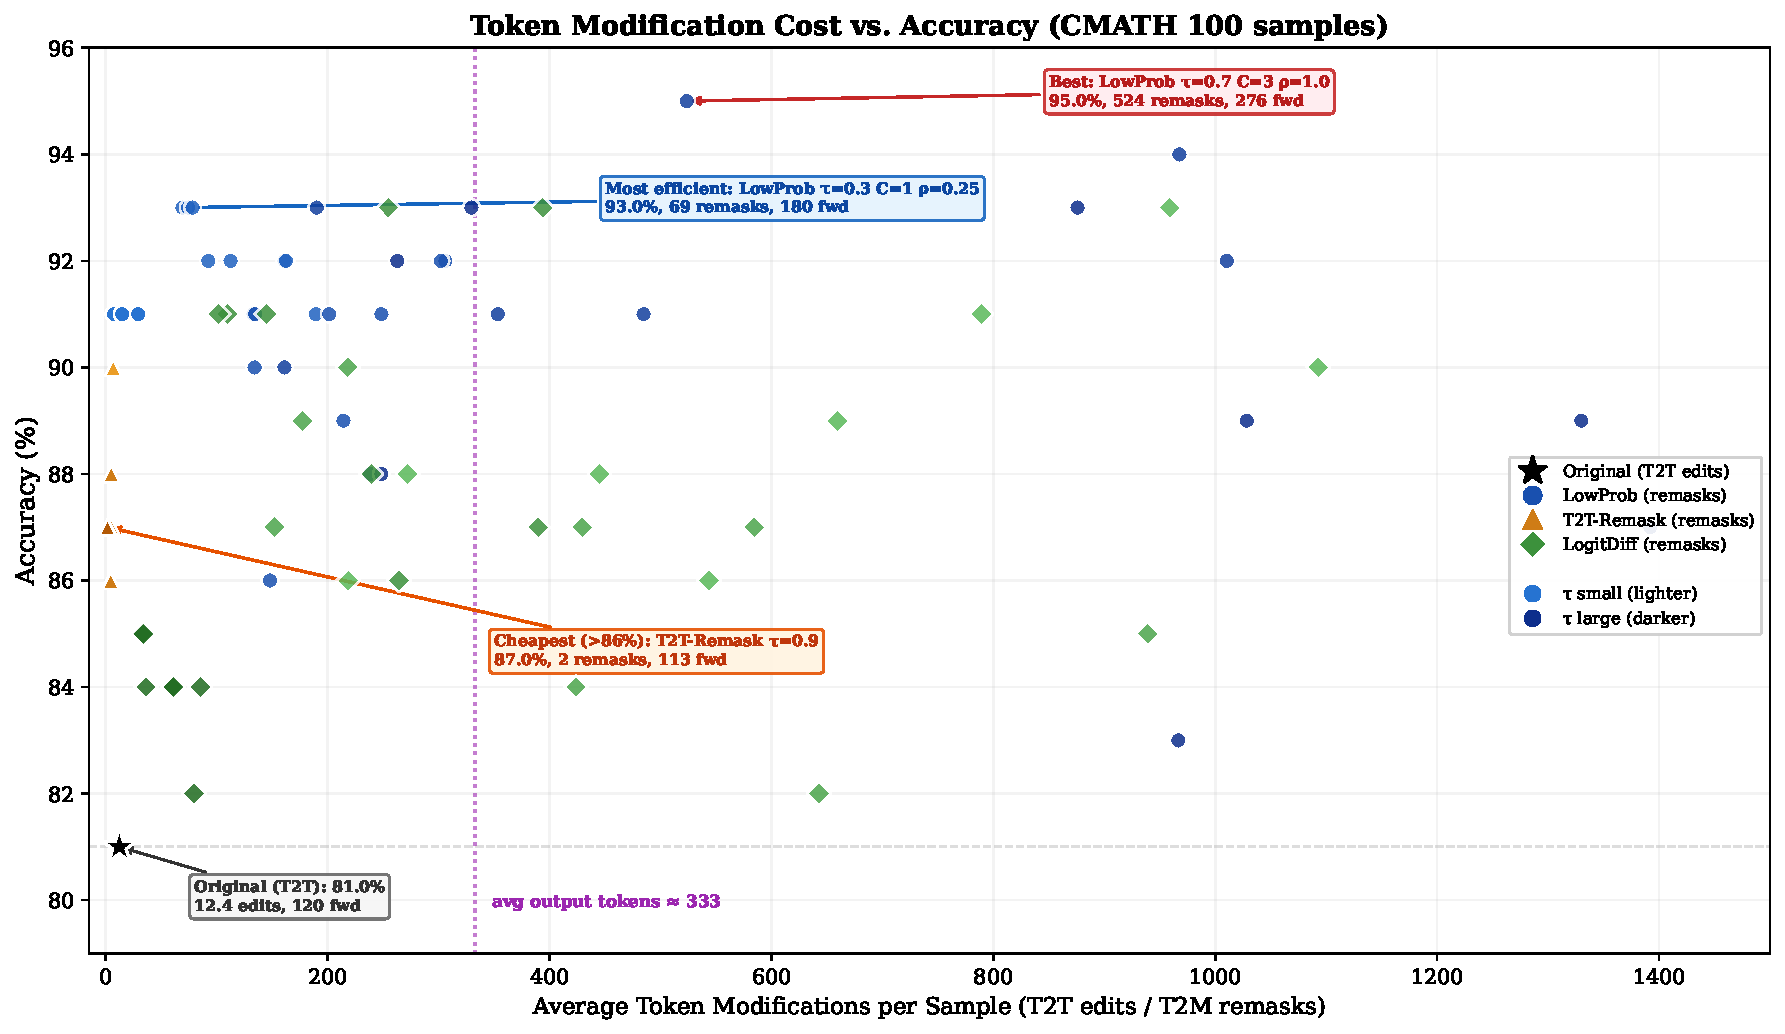
\includegraphics[width=\textwidth]{figures/ablation_tradeoff.pdf}
    \caption{\textbf{Token modification cost vs.\ accuracy.} Each point is one (strategy, $\tau$, $C_{\max}$, $\rho_{\max}$) configuration on CMATH (100 samples). The $x$-axis measures average token modifications per sample: T2T edits for the baseline, remasks for \TtoM{} strategies. Color shade encodes $\tau$ (lighter = smaller). The vertical dotted line marks the average output length (${\sim}334$ tokens). All \TtoM{} strategies surpass the T2T baseline (81\%, ${\star}$). \textbf{Most efficient}: \textsc{LowProb} $\tau{=}0.3$, $C{=}1$, $\rho{=}0.25$ (93\%, only 69.2 remasks). \textbf{Cheapest}: \textsc{T2T-Remask} $\tau{=}0.9$, $C{=}1$, $\rho{=}0.5$ (87\%, 1.7 remasks).}
    \label{fig:ablation}
\end{figure}

Several trends emerge:
\begin{itemize}[nosep,leftmargin=*]
    \item \textbf{All strategies improve over T2T.} Every \TtoM{} configuration exceeds the T2T baseline (81\%, 12.4 edits), confirming that on CMATH, remasking is preferable to token replacement across all tested hyperparameter configurations.
    \item \textbf{\textsc{LowProb} dominates.} Across all cost levels, \textsc{LowProb} achieves the highest accuracy. The most cost-efficient configuration ($\tau{=}0.3$, $C{=}1$, $\rho{=}0.25$) reaches 93\% with only 69.2 remasks.
    \item \textbf{\textsc{T2T-Remask} is cheapest.} With $\tau{=}0.9$, $C{=}1$, $\rho{=}0.5$, it triggers only 1.7 remasks per sample yet improves accuracy to 87\% (+6\%).
    \item \textbf{Over-remasking hurts.} Large $\tau$ (e.g., 0.9 for \textsc{LowProb}) combined with large $C_{\max}$ and $\rho_{\max}$ produces $>$1000 remasks per sample, degrading accuracy below 88\%. The safety mechanisms ($C_{\max}$, $\rho_{\max}$) are essential for preventing this.
\end{itemize}

\noindent Overall, the most cost-efficient configuration (\textsc{LowProb} $\tau{=}0.3$, $C{=}1$, $\rho{=}0.25$) adds only 69.2 remasks per sample---modest relative to the average output length of ${\sim}334$ tokens---while achieving a 12-point accuracy gain over \TtoT{}.

\subsection{Analysis}
\label{sec:analysis}

\paragraph{Last-mile token corruption: the dominant error mode.}
We conduct a systematic error analysis on CMATH (1,098 elementary math problems), where \TtoM{} achieves the largest gain ($+5.9\%$). Among the 194 errors made by \TtoT{}, \textbf{155 (79.9\%)} are \emph{last-mile token corruption}: the model's chain-of-thought reasoning arrives at the correct answer, yet the final extracted answer is corrupted during denoising. Only 39 errors (20.1\%) are genuine reasoning failures. Corruption takes several characteristic forms: \textbf{extra digits appended} ($18 \to 188$, 44 cases), \textbf{digits dropped} ($32 \to 2$, 26 cases), \textbf{answer marker repetition} (25 cases), and \textbf{single-digit substitution} (14 cases).

\TtoM{} remasking repairs \textbf{92 of 155} corruption cases (59.4\%), reducing total corruption errors from 155 to 91 ($\downarrow$41.3\%), while genuine reasoning errors remain virtually unchanged (39$\to$38). Table~\ref{tab:corruption} provides the full breakdown; representative examples are shown in Figure~\ref{fig:case_study} (Appendix~\ref{app:cases}).

\begin{table}[t]
\centering
\caption{Error breakdown on CMATH: \TtoT{} vs.\ \TtoM{}. ``Corruption'' = correct answer in reasoning chain but wrong final extraction.}
\label{tab:corruption}
\vspace{4pt}
\small
\begin{tabular}{lcccc}
\toprule
& \textbf{Total Errors} & \textbf{Corruption} & \textbf{Genuine Reasoning} & \textbf{Accuracy} \\
\midrule
\TtoT{} editing   & 194  & 155 ~(79.9\%)  & 39 ~(20.1\%)  & 82.3\% \\
\TtoM{} remasking  & 129  & ~91 ~(70.5\%)  & 38 ~(29.5\%)  & 88.3\% \\
\midrule
$\Delta$           & $-65$ & $-64$ ~($\downarrow$41.3\%) & $-1$ & $+5.9\%$ \\
\bottomrule
\end{tabular}
\end{table}

Among the 104 samples that \TtoM{} flipped from incorrect to correct, 92 (88.5\%) are corruption fixes and only 12 (11.5\%) reflect improved reasoning. Conversely, \TtoM{} introduces 39 new errors: 30 are new corruption cases, indicating that remasking occasionally destabilizes the denoising process at the answer boundary, and 9 are new reasoning errors where remasking alters the generation path---though both failure modes occur far less often than improvements.

The step-by-step token denoising trajectory for a representative example (DROP 160, gold = 857) is provided in Figure~\ref{fig:trajectory} (Appendix~\ref{app:trajectory}), showing per-token probabilities at each denoising iteration for both \TtoT{} and \TtoM{}.

%=============================================================================
\section{Conclusion}
\label{sec:conclusion}
%=============================================================================

We have identified fundamental limitations of Token-to-Token (\TtoT{}) editing in LLaDA2.1 and proposed Token-to-Mask (\TtoM{}) remasking as a principled, training-free replacement. By resetting suspected erroneous tokens to the mask state instead of replacing them with potentially incorrect alternatives, \TtoM{} purifies the generation context, converts systematic inference errors back to the model's native \mask{} noise type, and enables joint multi-position re-optimization through delayed commitment.

Our theoretical analysis provides a unified understanding of why mask tokens are strictly preferable to erroneous tokens as context, drawing parallels between the discrete and continuous diffusion settings. Three complementary error detection strategies---\textsc{LowProb}, \textsc{T2T-Remask}, and \textsc{LogitDiff}---offer flexibility in detecting different types of token-level errors. Experiments across 12 benchmarks show general improvements on tasks requiring precise token-level output, with the largest gain on mathematics; our error analysis reveals that last-mile token corruption accounts for 79.9\% of errors on CMATH, with \TtoM{} repairing 59.4\% of such corruptions.

\paragraph{Limitations.} Our approach is specific to the \TtoT{} editing mechanism in LLaDA2.1 and may not directly apply to dLLMs without such a mechanism. The theoretical analysis relies on the assumption that mask context is always preferable to erroneous context, which may not hold when error rates are very low. The safety mechanisms introduce hyperparameters ($C_{\max}$, $\rho_{\max}$) that may require task-specific tuning.

\paragraph{Future work.} A central finding of this work is the \emph{train--inference noise mismatch}: the random token perturbations used in \TtoT{} training differ fundamentally from the systematic, model-generated errors encountered at inference. While \TtoM{} mitigates this by resetting errors to the model's native \mask{} noise type, a more direct remedy would be to close this gap at the training level. Specifically, \emph{noise-aware continued training} could replace the random perturbations in the \TtoT{} training stream with realistic, model-generated errors---collected by running the model's own inference pipeline and recording the actual erroneous tokens that arise. Training on such ``real noise'' would expose the model to the systematic error patterns it will face at inference, potentially improving both \MtoT{} predictions under polluted context and \TtoT{} correction accuracy. This is complementary to our inference-time approach: \TtoM{} improves the correction \emph{mechanism}, while noise-aware training improves the model's \emph{robustness} to realistic errors.

Beyond this, combining \TtoM{} remasking with sampling-level remasking (e.g., ReMDM) could yield further improvements. Learning the remask threshold adaptively (e.g., via the PRISM framework) rather than using fixed heuristics is a promising direction. Extending the analysis to other dLLM architectures beyond LLaDA2.1 is also of interest.

\begin{ack}
Anonymous for review.
\end{ack}

\bibliographystyle{plainnat}
\bibliography{references}

%=============================================================================
\newpage
\appendix
\section{Benchmark Details}
\label{app:benchmarks}

Table~\ref{tab:benchmark_details} lists all benchmarks used in our evaluation with dataset details.

\begin{table}[h]
\centering
\caption{Benchmark details.}
\label{tab:benchmark_details}
\small
\begin{tabular}{llccc}
\toprule
\textbf{Category} & \textbf{Benchmark} & \textbf{Split} & \textbf{Samples} & \textbf{Metric} \\
\midrule
\multirow{3}{*}{Knowledge}
& GPQA-Diamond   & train & 198     & Accuracy    \\
& TriviaQA       & val   & 17,944  & EM / F1     \\
& MMLU-Pro       & test  & 12,032  & Accuracy    \\
\midrule
\multirow{4}{*}{Reasoning}
& HellaSwag      & val   & 10,042  & Accuracy    \\
& PIQA           & test  & 1,838   & Accuracy    \\
& DROP           & val   & 9,535   & EM / F1     \\
& BBH            & test  & 6,511   & Accuracy    \\
\midrule
\multirow{3}{*}{Math}
& CMATH            & test     & 1,098 & EM (numeric) \\
& AIME 2025        & --       & 30    & EM (integer) \\
& GSM Plus         & test     & 2,400 & EM (numeric) \\
\midrule
Coding
& HumanEval+ & --  & 164 & pass@1 \\
\midrule
Instruction
& IFEval         & test  & 541   & Prompt Strict Acc \\
\bottomrule
\end{tabular}
\end{table}

\section{Hyperparameter Details}
\label{app:hyperparams}

All remask-specific hyperparameters and their defaults are listed in the main text. Shared inference parameters follow LLaDA2.1 Q Mode: \texttt{threshold}$=0.7$, \texttt{editing\_threshold}$=0.5$, \texttt{block\_length}$=32$, \texttt{temperature}$=0.0$. The denoising inner loop runs until convergence (all masks filled and no edits/remasks triggered), not for a fixed number of steps.

\section{Representative Case Studies on CMATH}
\label{app:cases}

Figure~\ref{fig:case_study} shows a representative CMATH case from the corruption analysis in Section~\ref{sec:experiments}. The model performs correct arithmetic in its chain-of-thought, but \TtoT{} editing fails to prevent the final answer from being corrupted. \TtoM{} remasking, by resetting low-confidence tokens to \mask{} and re-predicting them, produces the correct final answer.

\begin{figure}[htp]
\centering
\small
\setlength{\fboxsep}{6pt}
\setlength{\fboxrule}{0.4pt}

\noindent\fbox{\parbox{0.96\textwidth}{%
\textbf{Leading digits dropped + answer marker repeated} \hfill Gold: \textbf{31}\\[3pt]
\textit{Q: Xiaofang is 8 years old and her mother is 39. How many years younger is Xiaofang than her mother?}\\[3pt]
\textbf{\TtoT{}}: \quad Reasoning: $39 - 8 = 31$ ~\checkmark \quad$\to$\quad ``The answer is the answer is \textcolor{red}{\textbf{1}}'' ~\ding{55}\\
\textbf{\TtoM{}}: \quad Reasoning: $39 - 8 = 31$ ~\checkmark \quad$\to$\quad ``The answer is \textcolor{teal}{\textbf{31}}'' ~\checkmark
}}

\caption{Representative CMATH case illustrating last-mile token corruption. Both methods produce correct chain-of-thought reasoning, but \TtoT{} editing generates a corrupted final answer---with a dropped leading digit and repeated answer marker---while \TtoM{} remasking outputs the correct result. The answer marker phrase is translated from the Chinese original for readability.}
\label{fig:case_study}
\end{figure}

\section{Token Denoising Trajectory}
\label{app:trajectory}

Figure~\ref{fig:trajectory} shows the full token-level denoising trajectory for the DROP 160 example (gold = 857) discussed in Section~\ref{sec:analysis}. Each cell displays the token and its model probability at that denoising step. The figure corresponds to Figure~\ref{fig:overview}(b) and provides the step-by-step detail of how \TtoT{} commits the error ``8''$\to$``6'' at $t{=}1$ while \TtoM{} remasks and recovers ``8'' at $t{=}2$.

\begin{figure}[htp]
    \centering
    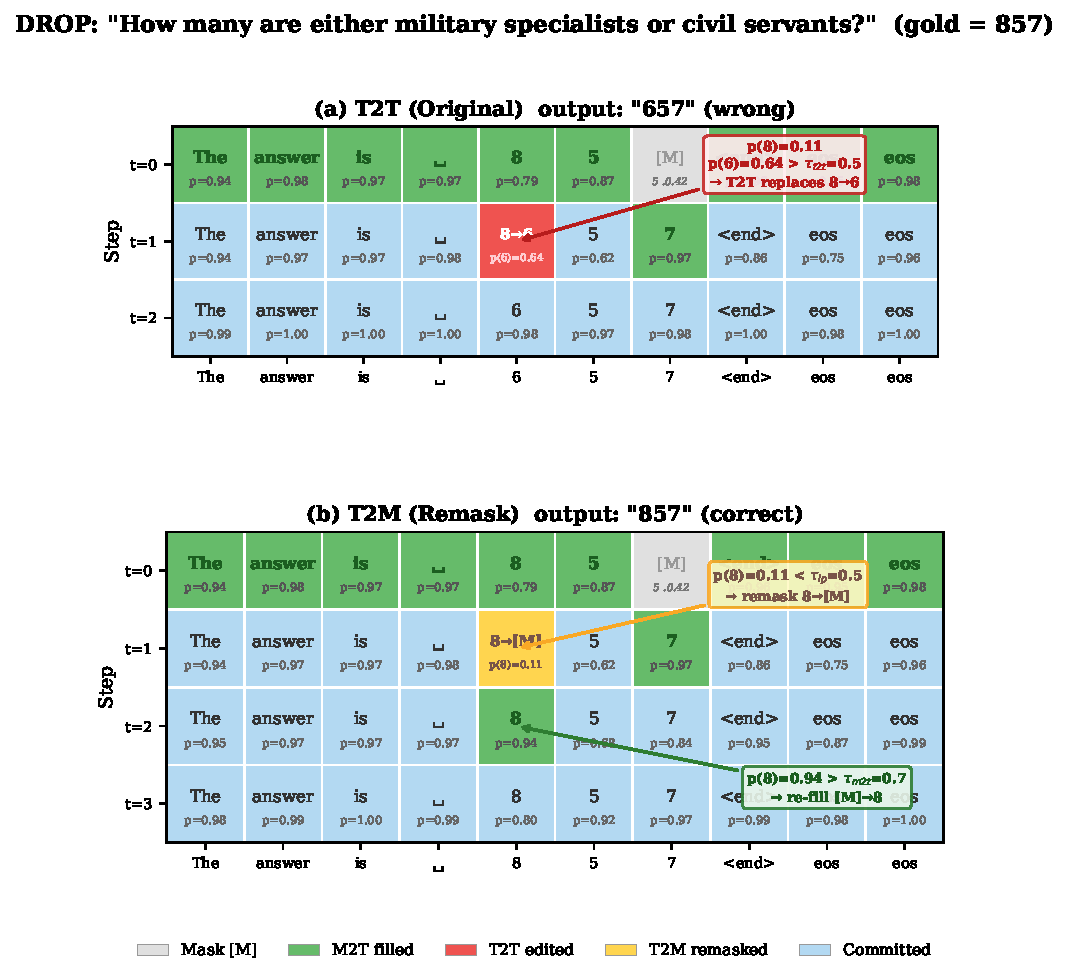
\includegraphics[width=\textwidth]{figures/trajectory_final.pdf}
    \caption{\textbf{Token denoising trajectory} for DROP example 160 (gold = 857). Each cell shows the token and its probability. \textbf{(a)} T2T: ``8'' ($p{=}0.11$) is replaced by ``6'' ($p{=}0.64$) at $t{=}1$, producing 657. \textbf{(b)} T2M: ``8'' is remasked at $t{=}1$, re-predicted as ``8'' ($p{=}0.94$) at $t{=}2$ under converged context (``5'', ``7'' committed), producing 857.}
    \label{fig:trajectory}
\end{figure}

%=============================================================================
\newpage
% \input{checklist}

\end{document}
